\section{Fundamentos de Mapas Geográficos}
	
	\subsection{Coordenadas}
	Coordenadas são usadas para expressar localizações no mundo. Existem vários sistemas de coordenadas diferentes. O usado pelo Google Maps é o Word Geodetic System 84 (WGS84), que é o mesmo sistema que o Global Position System(GPS) usa. As coordenadas são expressas usando o conceito de latitude e longitude. Onde latitude mede do sul ao norte e longitude me do oeste para o leste. No equador a latitude é 0. Isso significa que tudo abaixo do equador (hemisfério sul) possui uma latitude negativa, e tudo acima possui uma latitude positiva. Similarmente também existe uma linha zero para longitude. É conhecida como meridiano, e por razões históricas passa por Greenwich, Inglaterra. Cada posição que é localizada a leste desta linha tem um número positivo e tudo a oeste tem um número negativo\cite[4]{livroGoogleApiV3}. 
	
	A \autoref{fig-coordenadas} permite uma melhor observação desses conceitos:
	\begin{figure}[htb]
	\caption{\label{fig-coordenadas} O centro do mundo na latitude 0 e longitude 0 reside em algum lugar a oeste da costa da África}
	\begin{center}
	    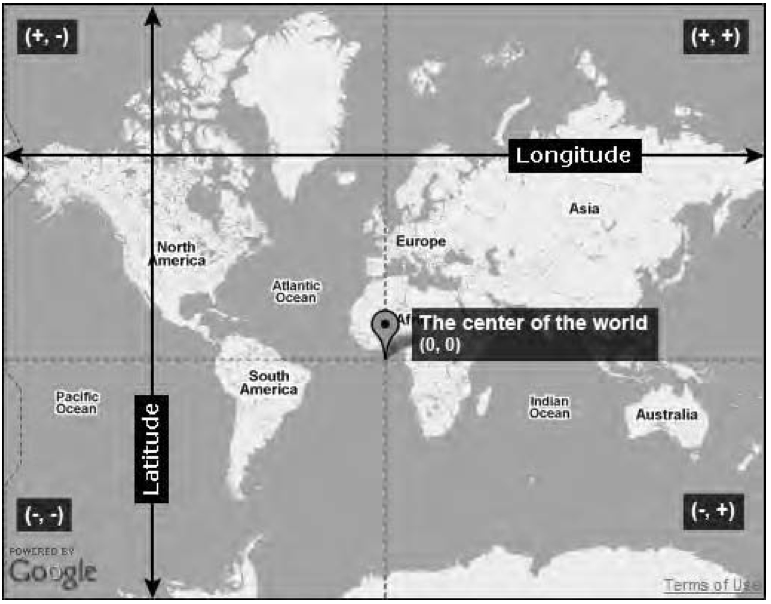
\includegraphics[scale=0.5]{goo-coordenadas}
	\end{center}
	\legend{Fonte: \cite[5]{livroGoogleApiV3}}
	\end{figure}
	
	
	Dessa forma é possível representar o mapa do mundo em uma imagem retangular que é projetada sobre o plano cartesiano.
	
	As coordenadas de latitude e longitude servem para localizar um ponto numa imagem retangular. Porém mapas também fornecem um terceira coordenada chamada Zoom. Esta  coordenada controla qual o tamanho da imagem que será usada para projetar o mapa sobre o plano cartesiano. Usualmente, um mapa com coordenada zoom, ou nível de zoom, igual a zero possui uma imagem de tamanho 256x256 pixels. A cada incremento da coordenada de zoom dobra-se o tamanho da imagem usada para representar o mapa, e consequentemente o nível de detalhes. De forma que que no zoom 2 a imagem do mapa do mundo terá 512x512 pixels, no zoom 3 1024x1024 e assim por diante. A \autoref{fig-zoomlevels} exemplifica esse processo:
	\begin{figure}[htb]
	\caption{\label{fig-zoomlevels} A cada incremento de zoom um mapa dobra a sua resolução de imagems}
	\begin{center}
	    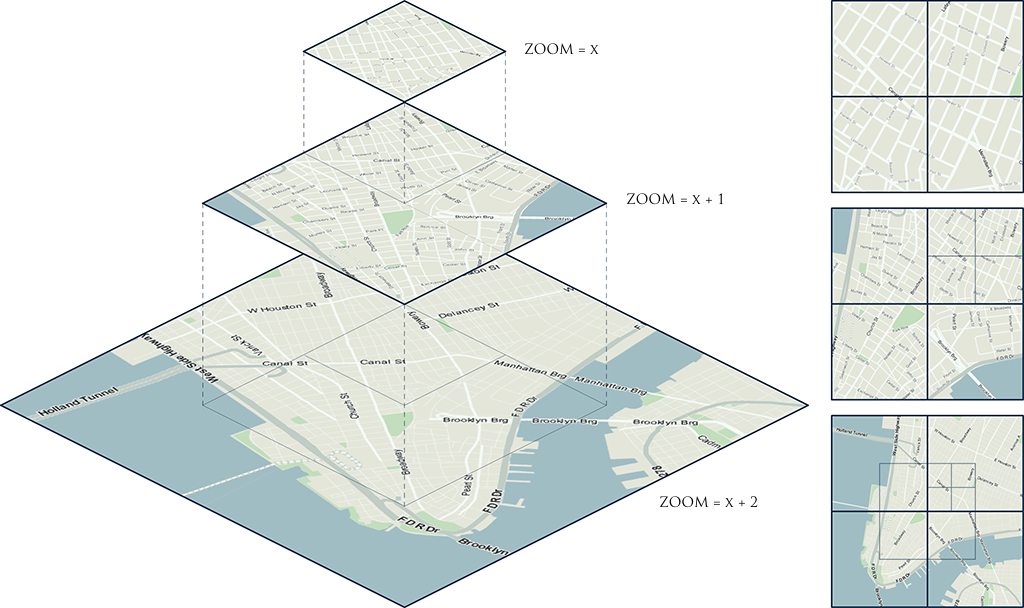
\includegraphics[scale=0.45]{tiles3d}
	\end{center}
	\legend{Fonte: http://workshops.opengeo.org/suiteintro/geowebcache/basics.html}
	\end{figure}

	Portanto para localizar uma posição  em um mapa web, precisamos de 3 coordenadas: latitude, longitude, zoom. Além disso, como o tamanho da imagem da projeção varia de acordo com o nível de zoom, o mapa precisa ajustar os valores das coordenadas latitude e longitude para que mantenham suas proporções para os diversos níveis de zoom.

	\subsection{Interação}
	Para fornecer uma melhor interação com os usuários, é comum encontrar mapas com 2 elementos básicos: Marcadores e Janelas de Informação.
	Marcadores são pequenas imagens que ficam sobrepostas ao mapa para indicar uma determinada posição no mapa. Em alguns, casos para facilitar a visualização de informações, usa-se de imagens diferentes para representar marcadores.
	Janelas de informação são usadas, geralmente, para detalhar alguma informação relativa a posição indicada pelo marcador e, em alguns casos, são exibidas quando o usuário clica em um marcador.
	A combinação desses dois elementos, nos mais diversos contextos, é responsável pela maioria das interações entre mapa e usuário.

\section{Estratégias para lidar com muitos marcadores}
	Um problema comum, ao lidarmos com mapas de crowdsourcing, é a enorme quantidade de marcadores necessários para representar os dados do mapa.Isto geralmente afeta a performance do mapa, pois quanto mais marcadores inserimos no mapa mais lento ele fica. 
	
	É difícil calcular exatamente qual o número máximo de marcadores que um mapa suporta antes de começar a ficar lento, pois a velocidade de exibição do mapa depende tanto do navegador quando do computador em que é exibido. Por exemplo, um mapa pode ser exibido bem rápido em um navegador como o Google Chrome e ao mesmo tempo ser lento quando exibido no Internet Explorer.\cite[177]{livroGoogleApiV3}
	
    Portanto, é necessário um estudo sobre as  estratégias para se lidar com o problema de exibição de muitos marcadores em um mapa. Em \cite[capítulo~9]{livroGoogleApiV3} o autor comenta sobre duas estratégias básicas para esse problema. A primeira e mais óbvia é reduzir o número de marcadores. A segunda estratégia consiste em agrupar os marcadores por algum grau de semelhança.
    
  \subsection{Reduzindo o número de marcadores}
  Existem muitos meios de se reduzir o número de marcadores, entre eles destaca-se as reduções via busca, filtro e otimização visual.
	\subsubsection{Busca}
	Para se reduzir  o número de marcadores exibidos no mapa pode-se fornecer um mecanismo de pesquisa ou busca no mapa. Dessa forma mesmo que o mapa possua milhões de marcadores, somente aqueles que satisfaçam os critérios da busca são exibidos.
	
	 \begin{figure}[htb]
	\caption{\label{fig-estrategiabusca}Busca como estratégia para redução do número de marcadores}
	\begin{center}
	    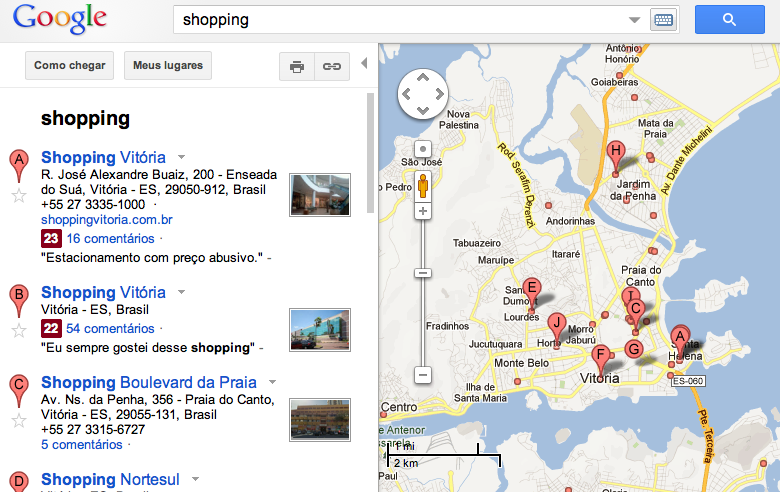
\includegraphics[scale=0.6]{estrategia-busca}
	\end{center}
	\legend{Fonte: http://maps.google.com}
	\end{figure}
	 
	 A \autoref{fig-estrategiabusca}  exemplifica bem isso, pois o google maps possui um catálogo enorme de informações, sobre regiões geográficas, se ele resolve-se mostrar todas essas informações ao mesmo tempo o mapa ficaria muito poluído, e praticamente inutilizável. Como ele implementa o mecanismo de busca isto não acontece . 
	
	\subsubsection{Filtro}
	De forma similar ao mecanismo de busca, um mapa também pode possuir um mecanismo para filtrar grupos de marcadores de acordo com algum critério de seleção do grupo. Dessa forma somente somente os marcadores que pertençam aos grupos marcados no filtro são exibidos no mapa.
	
	A \autoref{fig-estrategiafiltro} mostra um mapa com filtro a esquerda. Observa-se que apenas os marcadores dos grupos  "Student Housing" e "Food/Dining"  são exibidos no mapa.
	 \begin{figure}[htb]
	\caption{\label{fig-estrategiafiltro}Filtro como estratégia para redução do número de marcadores}
	\begin{center}
	    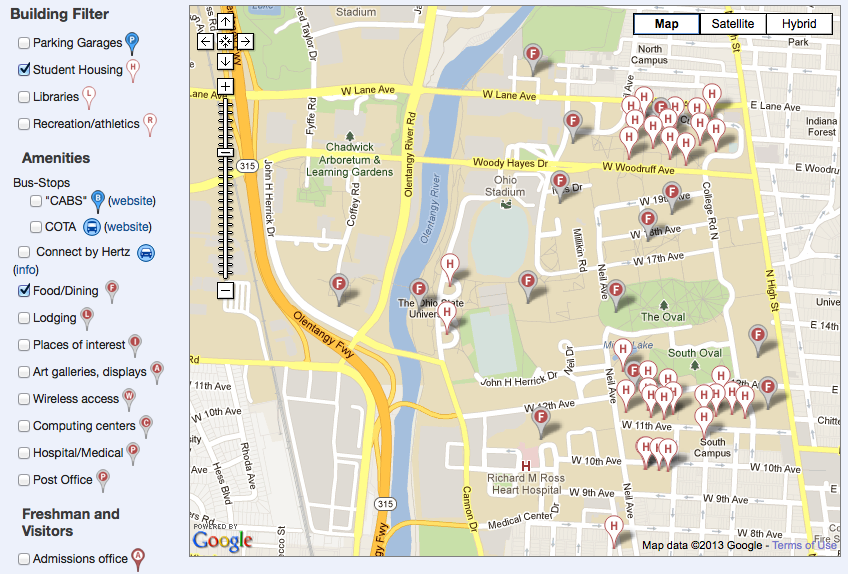
\includegraphics[scale=0.5]{estrategia-filtro}
	\end{center}
	\legend{Fonte: http://www.osu.edu/map/google.php}
	\end{figure}
	 
	\subsubsection{Otimização Visual}
	Nem sempre é preciso usar marcadores para representar dados de um mapa. Em alguns mapas faz mais sentido usar polígonos ou grupo de polígonos para representar um dado ao invés de simplesmente um ponto para o marcador. Por exemplo, ao exibir uma rota  num mapa não é necessário um marcador para cada vértice vértice da rota, pois para representar a rota precisa-se apenas desenhar uma linha passando por cada vértice.
	
	A \autoref{fig-otimizacao} mostra um exemplo desse tipo de otimização. Ela exibe, no mapa a esquerda, uma rota com marcadores em cada vértice do trajeto percorrido. No mapa a direita, ela exibe a mesma rota só que sem colocar marcadores nos vértices do trajeto, deixando apenas um marcador para exibir o ponto de início do trajeto.
	
	 \begin{figure}[htb]
	\caption{\label{fig-otimizacao}Otimização Visual como estratégia para redução do número de marcadores}
	\begin{center}
	    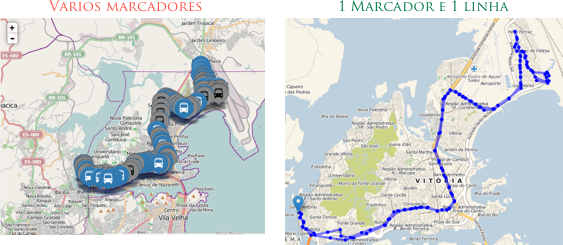
\includegraphics[scale=0.7]{estrategia-otimizacao}
	\end{center}
	\end{figure}
	
	
	

  \subsection{Agrupamento/Clustering}
  pagina 199 (google)
  
  	 
 pagina 198

 
 (pagina 88 ,silva, tabela 6, figura 93, figura 65 ())
ss
		\subsubsection{Por grelha}
		\subsubsection{Por distancia}
		\subsubsection{Por região}
		
\section{Algorítimos de agrupamento}
	\subsection{Métodos baseados em grelha}
		\subsubsection{WaveCluster}
	\subsection{Aplicações}
		\subsubsection{MarkerCluster}
		pagina 206 a 212
		\subsubsection{MarkerClustered}



\section{Planilhas eletrônicas e Mapas}
\subsection{O desafio chinês}
mostra o uso de planilhas pelo governo chines \cite{chinaPlanilha}
\subsection{Domínios de conhecimento}
Mostra a importância do uso de planilhas \cite{credinePlanilha} 
\subsection{Usando planilhas como fonte de dados para Mapas Geográficos}
Mostra \cite{lieberman2009spatio}